\documentclass[notitlepage]{report}
\usepackage{graphicx}
\usepackage{amsmath}
\usepackage{amssymb}
\usepackage[parfill]{parskip}
\newcommand\numberthis{\addtocounter{equation}{1}\tag{\theequation}}


\usepackage{titling}

\title{Desmos Polygonal Diagrams (draft)}
\author{Dan MacKinnon}

\begin{document}
\maketitle
\begin{abstract}
\noindent
Polygonal numbers, like the triangular, square, and pentagonal numbers, are closely identified with (or even defined in terms of) the diagrams that they are associated with. The functional approach provided by the Desmos graphing calculator provides fun and interesting ways of exploring number diagrams, like those associated with polygonal numbers. This short article provides one set of formulas that can be used to build polygonal number diagrams in Desmos.  
\end{abstract}

\section*{Polygonal numbers}
For a given $k \in \mathbb{Z}^+, k>2$, the $k$-polygonal numbers are a recursively defined integer sequence, as shown in Equation (\ref{eq:defn1}). 

\begin{align*}
    p_{k, 1} &= 1 \\
    p_{k,i} &= p_{k,i-1} + (k-2)i - (k-3)
    \numberthis
    \label{eq:defn1}
\end{align*}

For a term in the sequence $n = p_{k,i}$, $n$ dots can be arranged in a regular $k$-polygon built up of $i$ layers (traditionally referred to as \textit{gnomons}), as shown for the pentagonal numbers ($k=5$) of Figure (\ref{fig:pentagonals}). 

\begin{figure}[!htb]
    \centering
    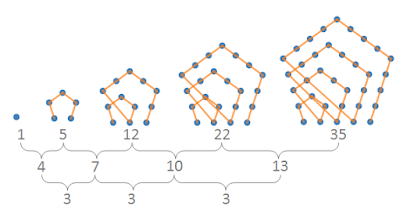
\includegraphics[width=0.5\linewidth]{pentagonal_numbers.PNG}
    \caption{The first few pentagonal numbers, showing first and second differences}
    \label{fig:pentagonals}
\end{figure}

If $n$ is the $i$th $k$-polygonal number, it can be drawn as a layered regular $k$-polygon with $i$ gnomon layers, as shown for the third pentagonal number $12$, $p_{5,3}=12$, in Figure (\ref{fig:gnomons}.

\begin{figure}[!htb]
    \centering
    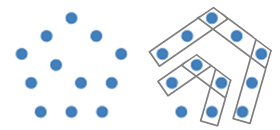
\includegraphics[width=0.5\linewidth]{pentagon_with_gnomon.PNG}
    \caption{Pentagonal number diagram $n=12$ with gnomons}
    \label{fig:gnomons}
\end{figure}

\section*{Placing any $n$ in a $k$-polygonal diagram}

Let $n,k \in \mathbb{Z}^{+}$, $n > 2$. We'd like to draw the $k-$polygonal number diagram "up to" $n$. If $n$ happens to actually be a $k-$polygonal number, this will be a complete diagram with $n$ dots in a layered $k$-polygon. Otherwise, this will be a diagram whose outer gnomon layer is incomplete.

Figure (\ref{fig:hexagonals}) shows hexagonal number ($k = 6$) diagrams for the numbers 15 and 26. Because 15 actually is a hexagonal number, the diagram is complete. The diagram for 26 shows an incomplete diagram, with an incomplete outer layer.

\begin{figure}[!htb]
    \centering
    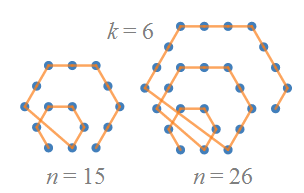
\includegraphics[width=0.5\linewidth]{hexagonal_and_no.PNG}
    \caption{Two hexagonal diagrams ($k = 6$), 15 is hexagonal, 26 is not}
    \label{fig:hexagonals}
\end{figure}


\subsection*{Finding the gnomon for $n$ and $k$}

The recursive definition for $p_{k,1}$ in Equation (\ref{eq:defn1} yields formulas stated as a summation (\ref{eq:summation}) and a direct calculation (\ref{eq:quad}).

\begin{equation}
    p_{k,i} = \sum^{i}_{j=1}\left[(k-2)j-(k-3)\right]
    \label{eq:summation}
\end{equation}

\begin{equation}
    p_{k,i} = \frac{(k-2)i(i+1)}{2} - (k-3)i
    \label{eq:quad}
\end{equation}

Applying the quadratic formula to solve $n-p_{k,i}=0$ provides us with

\begin{equation}
    g\left(n,k\right)=\frac{\left(k-4\right)+\sqrt{\left(k-4\right)^{2}+8n\left(k-2\right)}}{2\left(k-2\right)}
     \label{eq:quadform}
\end{equation}

This allows us to identify the preceding and current gnomon layers for a given $n$, along with a binary function determining if a given $n$ is a polygonal number.

\begin{align}
    g_{previous}\left(n,k\right) &= \text{floor}\left(g\left(n\right)\right) \\
    g_{current}\left(n,k\right) &= \text{ceil}\left(g\left(n\right)\right)    
    \label{eq:prev-and-current}
\end{align}

\begin{equation}
    \text{isPoly}\left(n\right) = 1 - \left[ g_{current}\left(n,k\right) - g_{previous}\left(n,k\right) \right]
    \label{eq:isPoly}
\end{equation}

Equation (\ref{eq:isPoly}) is equivalent to (\ref{eq:isPoly2}).

\begin{equation}
 \text{isPoly}\left(n,k\right) =
    \begin{cases}
      0 & \text{if $n$ is not $k$-polygonal}\\
      1 & \text{if $n$ is $k$-polygonal}\\
    \end{cases} 
    \label{eq:isPoly2}
\end{equation}

\section*{Drawing the diagram}
Following this standard approach, to draw up to a given number $n$ in a $k$-polygonal diagram, you determine which gnomon layer it lies in, how far along the gnomon layer it is, and what side of the gnomon it is on. The gnomon layer for $n$ tells us where to start: we just need to count up to the layer along angle that is determined by $k$. If we know how far along in the layer it is, we know how many dots to move along before plotting our point. And finally, if we know which side it is on, we know how many turns to make along the way.

As mentioned, the angle needed in drawing these diagrams is completely determined by which type of polygonal number we are drawing. The shape of the diagram is determined by the angles in a regular $k$-gon. Define $a_{ngle}$ as in equation (\ref{eq:angle}).

\begin{equation}
    a_{ngle}=\left(\pi-((k-2)*(\pi/k))\right)
\label{eq:angle}
\end{equation}


$N$ is the ordered tuple $N=\left[1,\ ...\ ,n\ \right]$. Define the point $\left(x_{kn}\left(N\right),y_{kn}\left(N\right)\right)$ according to the formulas that follow.

\begin{equation}
x_{kn}\left(l\right)=-g_{nomon}\left(l\right)\cos\left(a_{ngle}\right)-\sum_{j=1}^{g_{depth}\left(l\right)}\cos\left(s_{k}\left(j,l\right)\cdot a_{ngle}\right)
\end{equation}

\begin{equation}    y_{kn}\left(l\right)=g_{nomon}\left(l\right)\sin\left(a_{ngle}\right)+\sum_{j=1}^{g_{depth}\left(l\right)}\sin\left(s_{k}\left(j,l\right)\cdot a_{ngle}\right)
\label{eq:yformula}
\end{equation}

The formulas for $x_{kn}$ and $y_{kn}$ express the idea of placing the point corresponding to the current polygonal number at the right spot in the correct gnomon layer for that number, as shown in Figure (\ref{fig:yannotated}).

% \begin{figure}
%     \centering
%     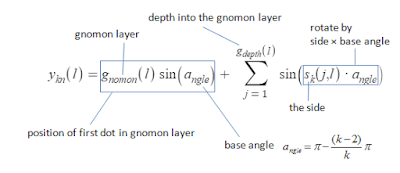
\includegraphics[width=0.5\linewidth]{annotated_eqn.PNG}
%     \caption{Formula for $y_{kn}$, annotated}
%     \label{fig:yannotated}
% \end{figure}


\begin{equation}
s_{k}\left(j,l\right)=\left(\text{ceil}\left(\frac{j}{g_{size}\left(l\right)}\left(k-2\right)\right)+1\right)
\end{equation}

\begin{equation}
g_{size}\left(l\right)=g_{nomon}\left(l\right)\cdot\left(k-2\right)+1
\end{equation}

\begin{equation}
    g_{depth}\left(l\right)=\sum_{o=1}^{l-1}\left(\operatorname{floor}\left(\frac{g_{nomon}\left(o\right)}{g_{nomon}\left(l\right)}\right)\right)
\end{equation}

\begin{equation}
    g_{nomon}\left(l\right)=\sum_{i=1}^{l-1}p_{olygonal}\left(i\right)
\end{equation}

\begin{equation}
    p_{olygonal}\left(l\right)=1-\left(p_{up}\left(l\right)-p_{down}\left(l\right)\right)
\end{equation}

\begin{equation}
p_{down}\left(l\right)=\operatorname{floor}\left(p_{verse}\left(l\right)\right)
\end{equation}

\begin{equation}
p_{up}\left(l\right)=\operatorname{ceil}\left(p_{verse}\left(l\right)\right)
\end{equation}

One method of finding out the gnomon layer we are in is to use a formula for computing polygonal numbers along with the quadratic formula. This approach is expressed in equations (\ref{eq:quadform}) and (\ref{eq:determinant}).

\begin{equation}
    p_{verse}\left(l\right)=\frac{\left(k-4\right)+\sqrt{D\left(l\right)}}{2\left(k-2\right)}
     \label{eq:quadform}
\end{equation}

\begin{equation}
    D\left(l\right)=\left(k-4\right)^{2}+8l\left(k-2\right)
    \label{eq:determinant}
\end{equation}

\section{building with gnomons}

Comparing the listing for the hexagonal numbers with the diagrams above, you can see how the sequences are built diagrammatically. In general, beginning with a single dot, k-sided polygons are built by adding layers (called gnomons) consisting of k-2 segments, with each segment of the gnomon having one more dot than the segments of the previous layer. In this way, the nth gnomon consists of segments each n dots long, but with k-3 dots shared by adjoining segments (the corners).




\end{document}
